\chapter{Analisi dei requisiti} \label{chapter:ads}
Allo stato attuale, la gestione della rendicontazione delle ore di lavoro di ogni dipendente viene effettuata mediante un foglio di calcolo Excel, compilato in ogni sua parte, inserendo nome, cognome e orario di lavoro svolto giornalmente. Successivamente, alla fine di ogni mese, il dipendente spedisce tale file via email alla segreteria e al proprio responsabile di sede per l'approvazione. A seguito di un esito positivo viene effettuato il calcolo del salario mensile e quindi l'emissione dello stesso.

Le specifiche fornite inizialmente riguardano perlopiù funzionalità che tale prodotto deve fornire e il tipo di informazioni che deve essere in grado di gestire. Il sistema che s'intende realizzare vuole rendere fruibile il processo di scambio ed elaborazione delle informazioni appena descritto, mediante un prodotto software che ne semplifichi e ne automatizzi alcuni aspetti. Tali specifiche sono state poi raffinate, con un'analisi dei requisiti approfondita, anche grazie alla comunicazione con l'utente finale. Inoltre, in seguito all'analisi dei requisiti, viene presentata l'analisi tecnica atta a spiegare le scelte di progettazione ed implementazione. 

\section{Specifiche generali}
Formalmente le funzionalità principali richieste sono le seguenti:
\begin{enumerate}
    \item assegnamento di un'utenza, ossia nome utente e password, per effettuare l'accesso.
    \item inserimento, da parte del dipendente, dei dati utili alla rendicontazione mensile dell'attività lavorativa;
    \item invio del rendiconto lavorativo mensile, per approvazione da parte del proprio responsabile;
    \item verifica e validazione di tale rendiconto;
\end{enumerate}
Ognuna di queste è stata poi analizzata singolarmente per ricavare nel dettaglio i requisiti necessari ed, eventualmente, delle relative funzionalità aggiuntive. Vengono presentati di seguito i requisiti funzionali e non funzionali rilevati durante l'analisi.

\section{Requisiti funzionali}
Il software in analisi deve garantire un accesso protetto all'area riservata dell'utente. Per accedere esso inserisce username e password e, qualora i dati inseriti fossero errati, il sistema mostra una errore e non consente l'accesso. \\
Nel momento in cui si accede all'area personale è prevista una sezione in cui è possibile inserire le ore di lavoro, per ogni singolo giorno lavorativo del mese corrente. Per quanto riguarda l'assenza totale o parziale per una o più giornate, si potrà indicare il numero di ore di permesso usufruite e nel caso specifico di assenza totale, quindi per l'intera giornata lavorativa, sarà inibito l'inserimento del numero di ore da parte dell'utente. È importante che in corrispondenza di ogni inserimento sia possibile specificare il codice relativo all'attività svolta in quella giornata. Tale codice viene generato dal responsabile di sede e reso disponibile nell'area personale dell'impiegato. Inoltre l'utente può compilare parzialmente il mese in corso e salvarne lo stato. A quel punto il sistema memorizzerà fisicamente i dati inseriti e quando si verifica un nuovo accesso, ripristinerà la compilazione precedente, permettendone la modifica, la cancellazione oppure l'invio definitivo. Una volta inviato il timesheet, viene impedita l'ulteriore modifica, o cancellazione, dei dati inviati e non è possibile effettuare un nuovo invio. \\
L'applicazione fornisce altresì una funzionalità per la consultazione dei timesheet relativi ai mesi precedenti e permette di scaricarli localmente in un formato Excel (\texttt{.xls}). \\
Accedendo con l'utenza manager si possono generare dei codici, cosiddetti \textit{commesse}, e assegnarli ad uno specifico impiegato. Non può verificarsi un assegnamento della stessa commessa a più impiegati, poiché questa identifica la mansione svolta in relazione con il cliente e il relativo progetto.\\
In aggiunta all'utenza manager, il sistema permette all'utente in questione la visualizzazione di tutti i timesheet inviati dai relativi dipendenti appartenenti alla sede cui esso afferisce. Una volta selezionato un timesheet e controllatone la correttezza dei dati, il manager può eseguirne l'approvazione o il rigetto, rispettivamente se i dati inseriti sono coerenti con l'attività svolta in quel determinato mese oppure sono errati. Qualora si verificasse un rigetto, il sistema provvederà a riabilitare la modifica del timesheet nell'area personale del dipendente. Infine, ogni volta che si verifica un assegnamento di una commessa oppure l'avvenuta approvazione o rigetto del timesheet, occorre notificarlo all'impiegato nell'apposita sezione. Viene inoltre mostrata una notifica anche nel caso in cui il dipendente non abbia ancora effettuato l'invio entro il terzultimo giorno del mese corrente.

\section{Casi d'uso}
I casi d'uso sviluppati riguardano i processi di login, di compilazione del timesheet (ts) da parte dell'impiegato e di validazione dello stesso da parte dell'utente manager, i quali vengono riportati nel diagramma in figura. \ref{fig:usecase}. 

\begin{figure}[H]
	\centering
	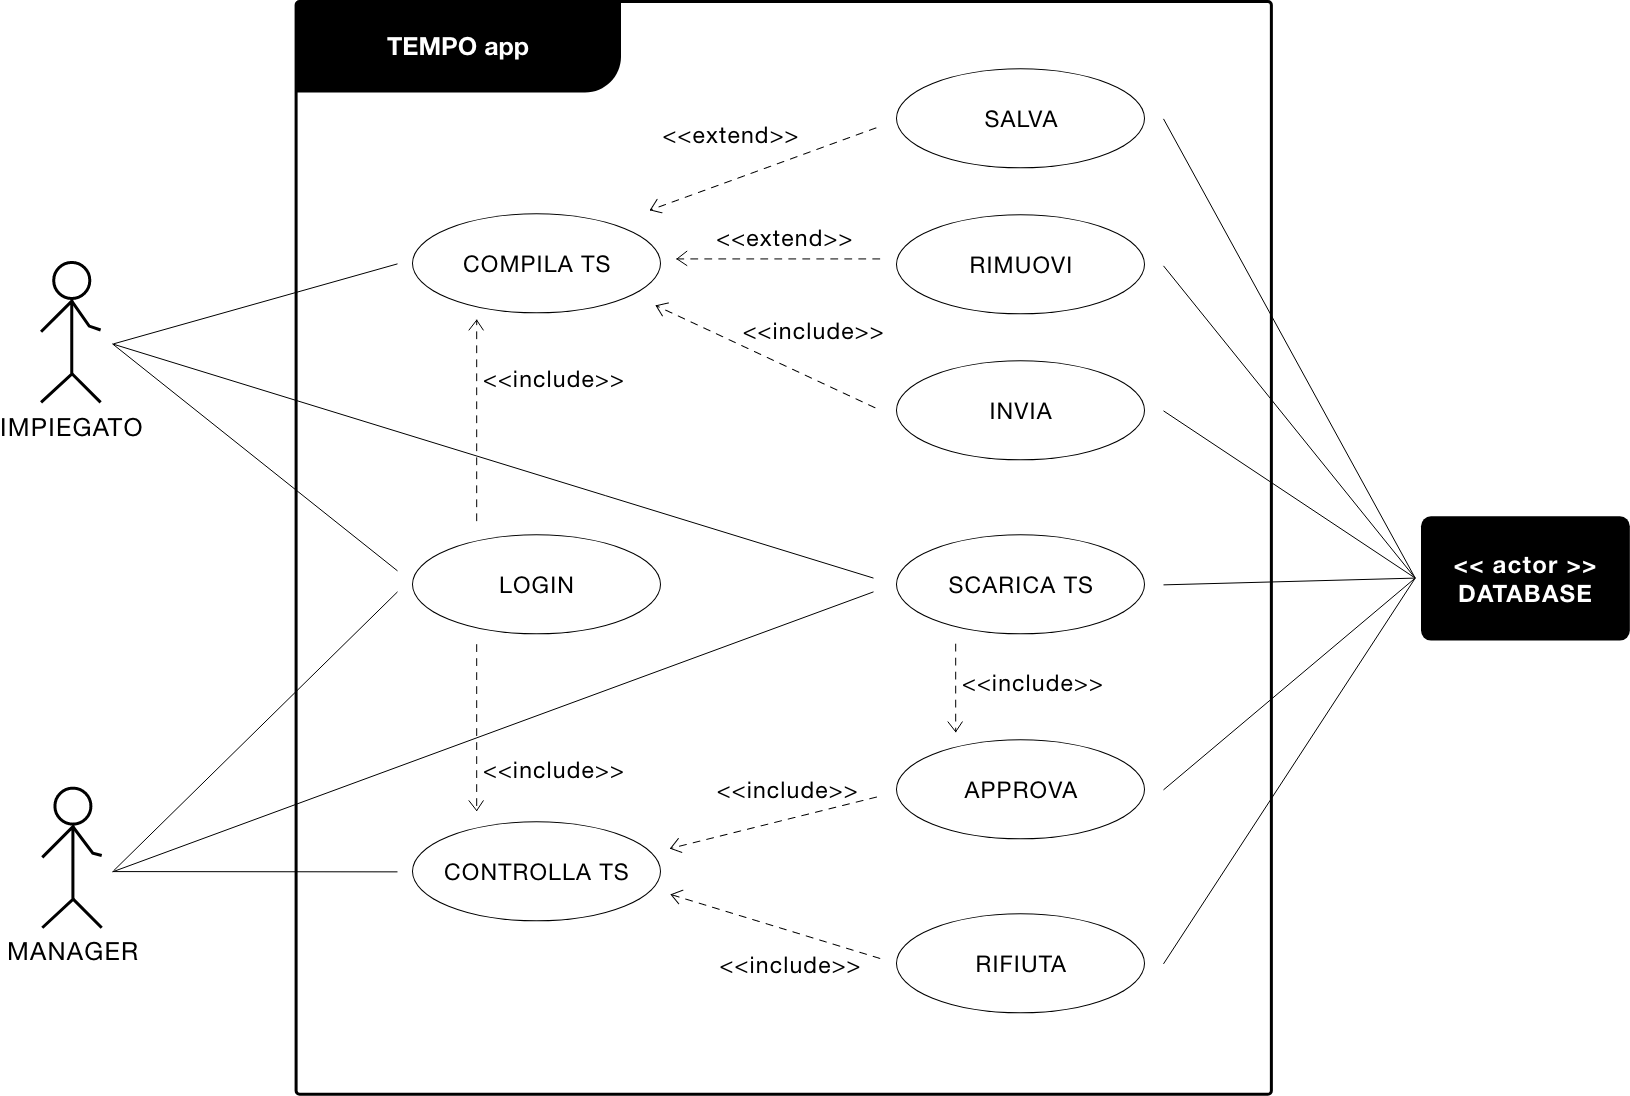
\includegraphics[width=1\linewidth]{ucd.png}
	\caption{Diagramma dei casi d'uso.}
	\label{fig:usecase}
\end{figure}

All'interno delle ultime due macro-funzionalità citate, ne sono comprese altre. La compilazione del timesheet viene estesa con l'operazione di salvataggio, ossia la memorizzazione fisica dei vari inserimenti effettuati dall'utente, e con l'operazione di rimozione, ovvero la cancellazione dei dati memorizzati mediante l'operazione precedente di salvataggio; e infine include l'invio, che avviene nel momento in cui l'utente decide che la compilazione è completata. Per quanto riguarda il controllo da parte del manager, esso comprende l'approvazione oppure il rigetto del timesheet inviato. Infine, nel momento in cui si verificano invio e conseguente approvazione, sarà disponibile la funzionalità che permetterà lo scaricamento in locale del file Excel.

\subsection{Login utente}
\textbf{Nome}: Login.\\
\textbf{Portata}: Tempo.\\
\textbf{Livello}: Obiettivo utente.\\
\textbf{Attore primario}: Impiegato, Manager, Azienda.\\
\textbf{Parti interessate e interessi}: Utente (Impiegato, Manager, Azienda), vuole effettuare l'accesso all'applicazione.\\
\textbf{Pre-condizioni}: L'utente è già stato registrato.\\
\textbf{Garanzia di successo}: L'utente si autentica e accede alla sua area personale.\\
\textbf{Scenario principale di successo}:
\begin{enumerate}
    \item L'utente avvia l'applicazione.
    \item Il sistema visualizza i campi in cui inserire le credenziali di accesso.
    \item L'utente inserisce username e password.
    \item Il sistema verifica la correttezza dei dati inseriti.
    \item Il sistema autentica l'utente e visualizza la sua area personale.
\end{enumerate}

\begin{figure}[H]
	\centering
	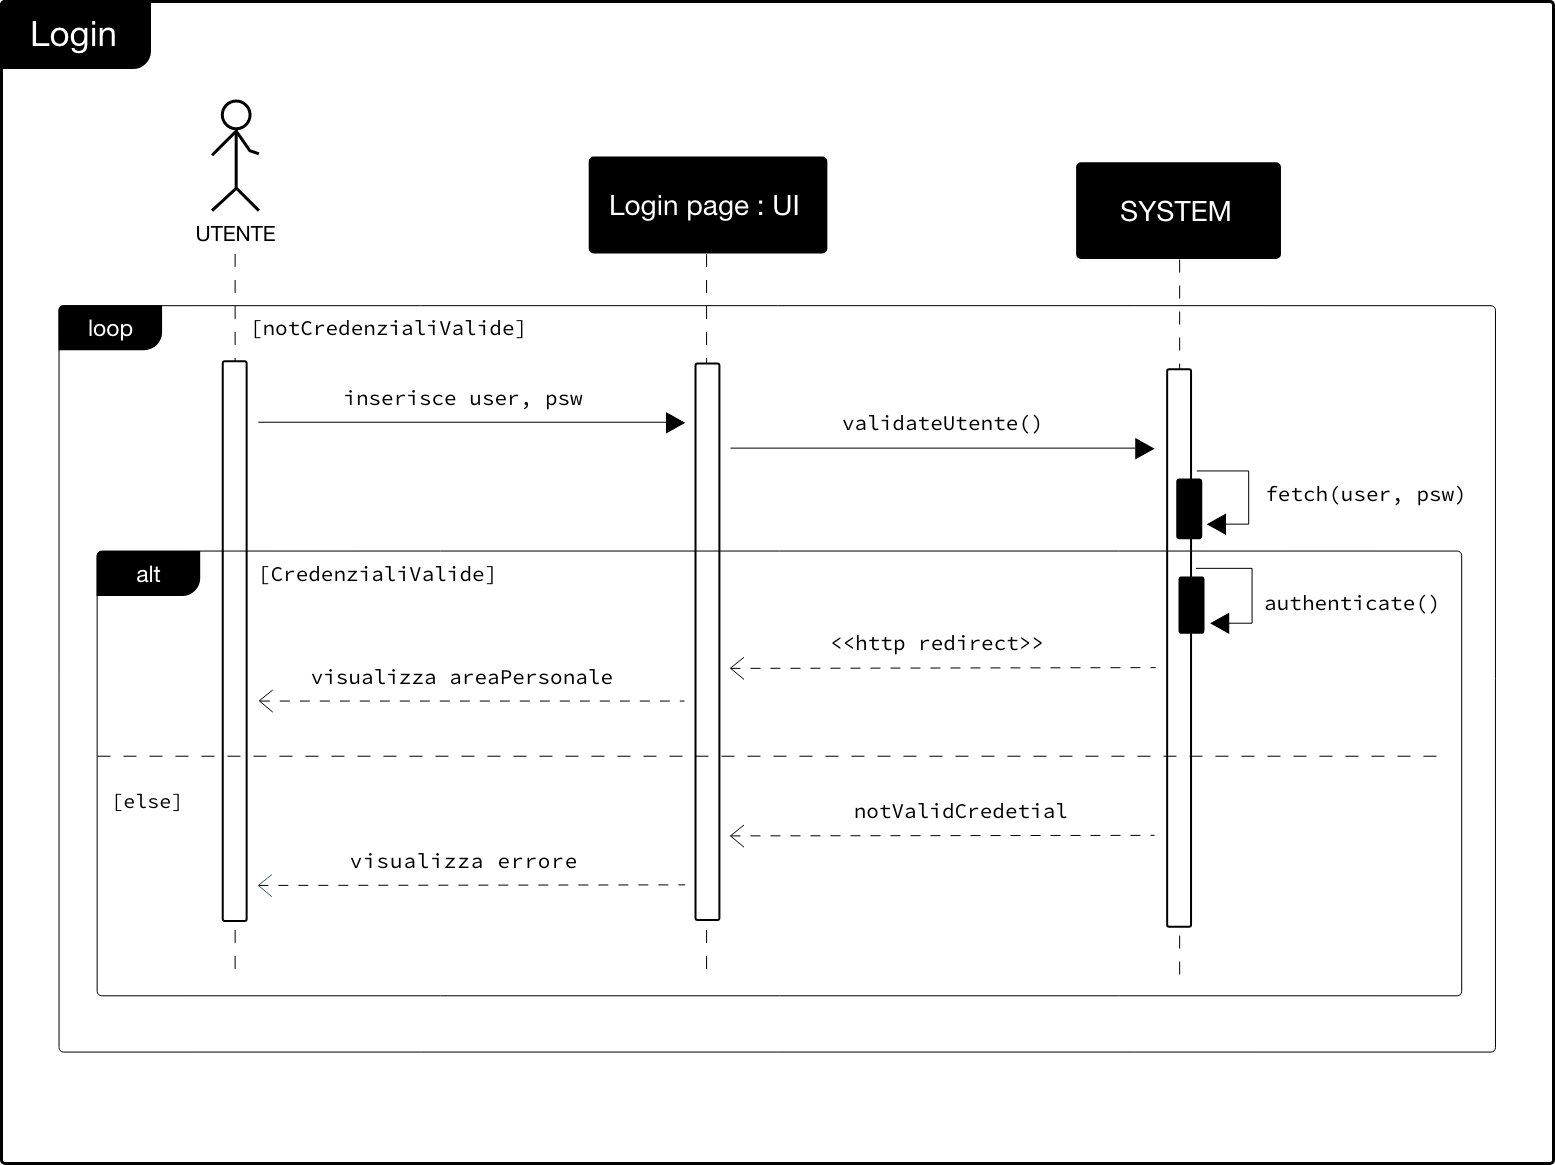
\includegraphics[width=1\linewidth]{SD_Login.png}
	\caption{Diagramma di sequenza relativo al login utente.}
	\label{fig:sd_login}
\end{figure}

\subsection{Compilazione timesheet}
\textbf{Nome}: Compila ts.\\
\textbf{Portata}: Tempo.\\
\textbf{Livello}: Obiettivo utente.\\
\textbf{Attore primario}: Impiegato.\\
\textbf{Parti interessate e interessi}: Impiegato, vuole compilare il timesheet indicando le ore di lavoro giornaliere, eventuali giorni di permesso/ferie e/o malattia.\\
\textbf{Pre-condizioni}: L'impiegato deve essere registrato e aver effettuato il login.\\
\textbf{Garanzia di successo}: L'impiegato annota correttamente le ore di lavoro giornaliere e il manager di sede può consultarle per l'eventuale approvazione.\\
\textbf{Scenario principale di successo}:
\begin{enumerate}
    \item L'impiegato sceglie il mese d'interesse nell'apposito calendario.
    \item L'impiegato seleziona uno fra i codici commessa disponibili.
    \item L'impiegato compila la tabella per la prima volta, inserendo le ore di lavoro effettuate per ogni giornata e/o inserendo eventuali giorni di permesso/malattia.
    \item L'impiegato termina la compilazione del mese selezionato e invia il timesheet.
    \item Il sistema registra i dati inseriti dall'utente.
    \item Il sistema mostra un messaggio di completamento dell'operazione.
    \item Il sistema disabilita la modifica al timesheet.
\end{enumerate}
\textbf{Estensioni}: \\
3a. L'impiegato aveva già salvato una compilazione parziale:
\begin{enumerate}
    \item L'impiegato procede con la compilazione del mese selezionato in precedenza.
    \item L'impiegato termina la compilazione del mese selezionato e invia il timesheet. 
    \item Il sistema registra i dati inseriti dall'utente.
    \item Il sistema mostra un messaggio di conferma.
    \item Il sistema disabilita la modifica al timesheet.
\end{enumerate}
3b. L'impiegato aveva già salvato una compilazione parziale e decide di eliminarla:
\begin{enumerate}
    \item L'impiegato rimuove il timesheet precedentemente salvato.
    \item Il sistema cancella tutti i dati relativi a quella compilazione.
    \item Il sistema mostra un messaggio di conferma.
    \item L'impiegato inizia una nuova compilazione.
\end{enumerate}
4a. L'impiegato salva il modulo senza inviarlo:
\begin{enumerate}
    \item Il sistema salva la compilazione e mantiene i dati per la prossima sessione.
    \item Il sistema mostra un messaggio di conferma.
\end{enumerate}

\begin{figure}[H]
	\centering
	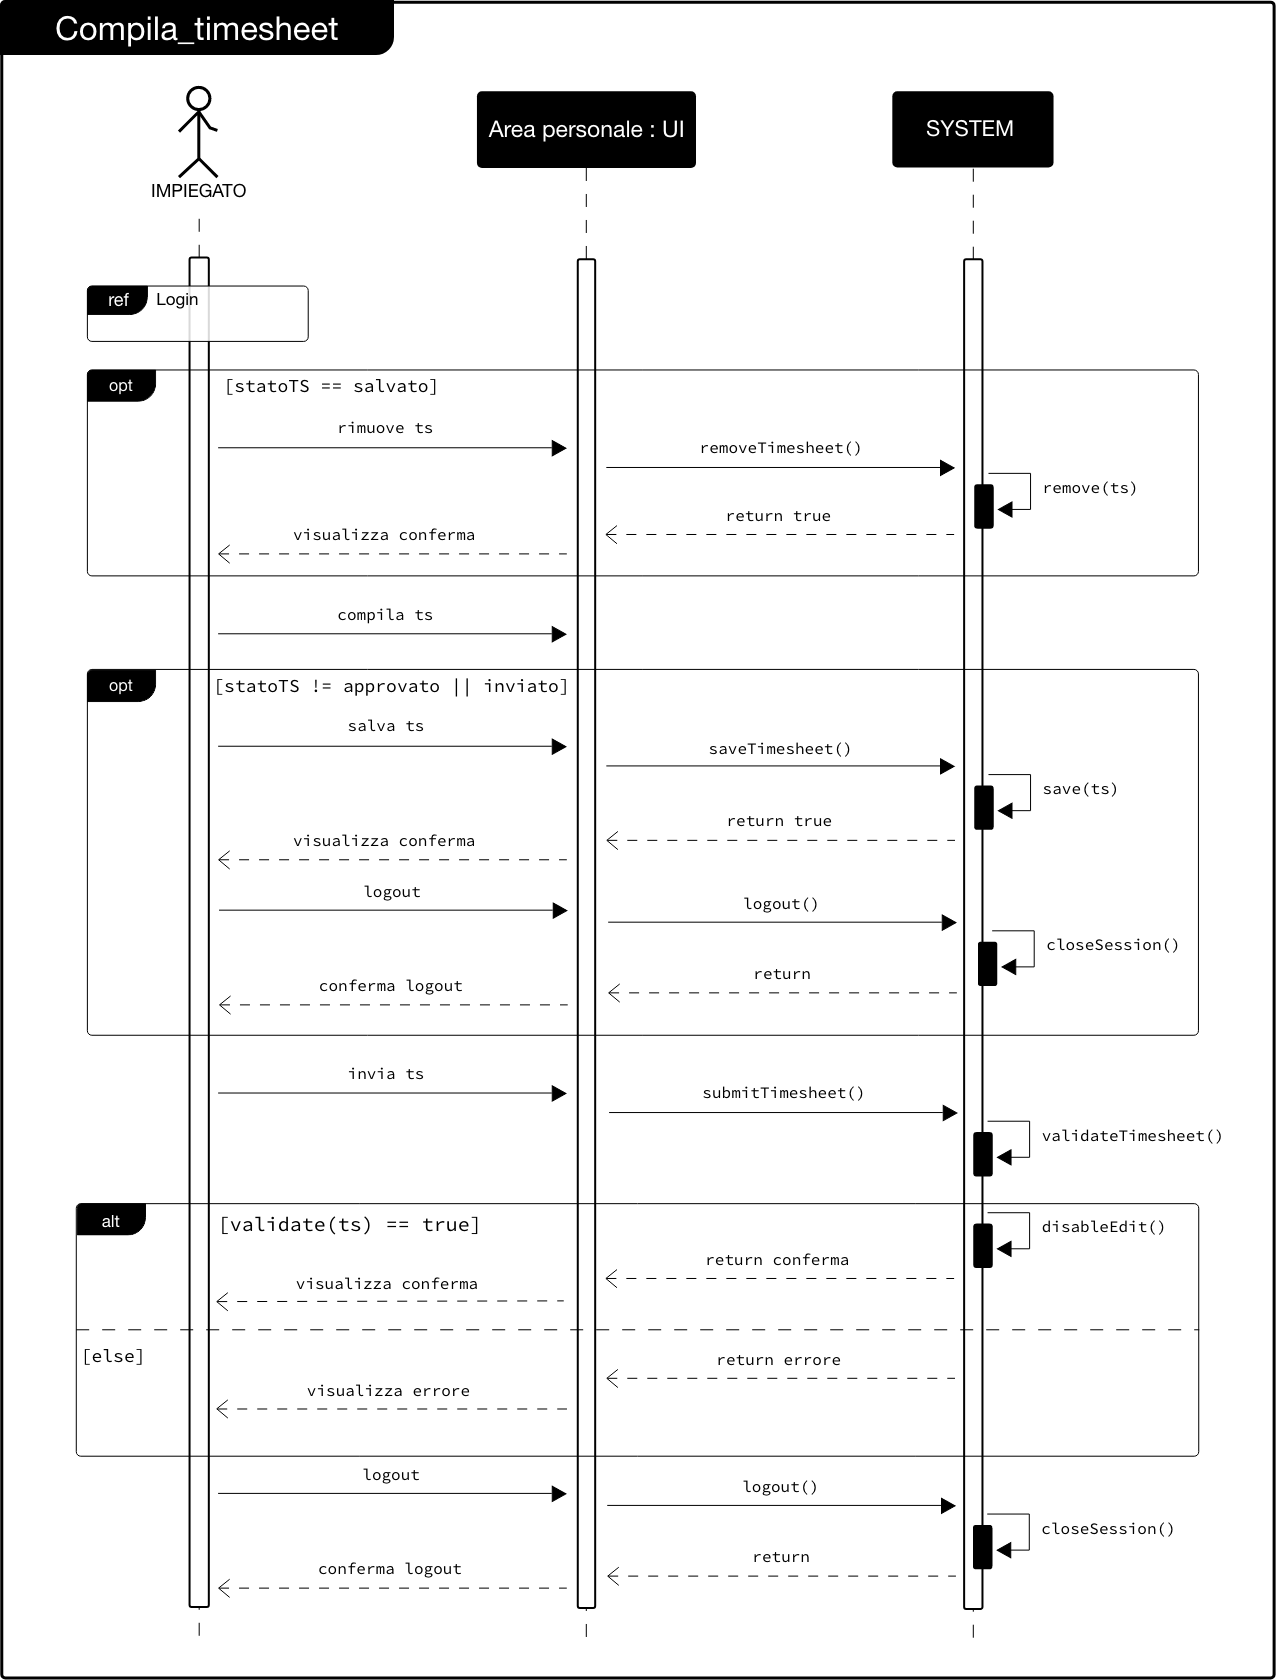
\includegraphics[width=1\linewidth]{SD_Compila_ts.png}
	\caption{Diagramma di sequenza relativo alla compilazione del timesheet.}
	\label{fig:sd_compilats}
\end{figure}

\begin{figure}[H]
	\centering
	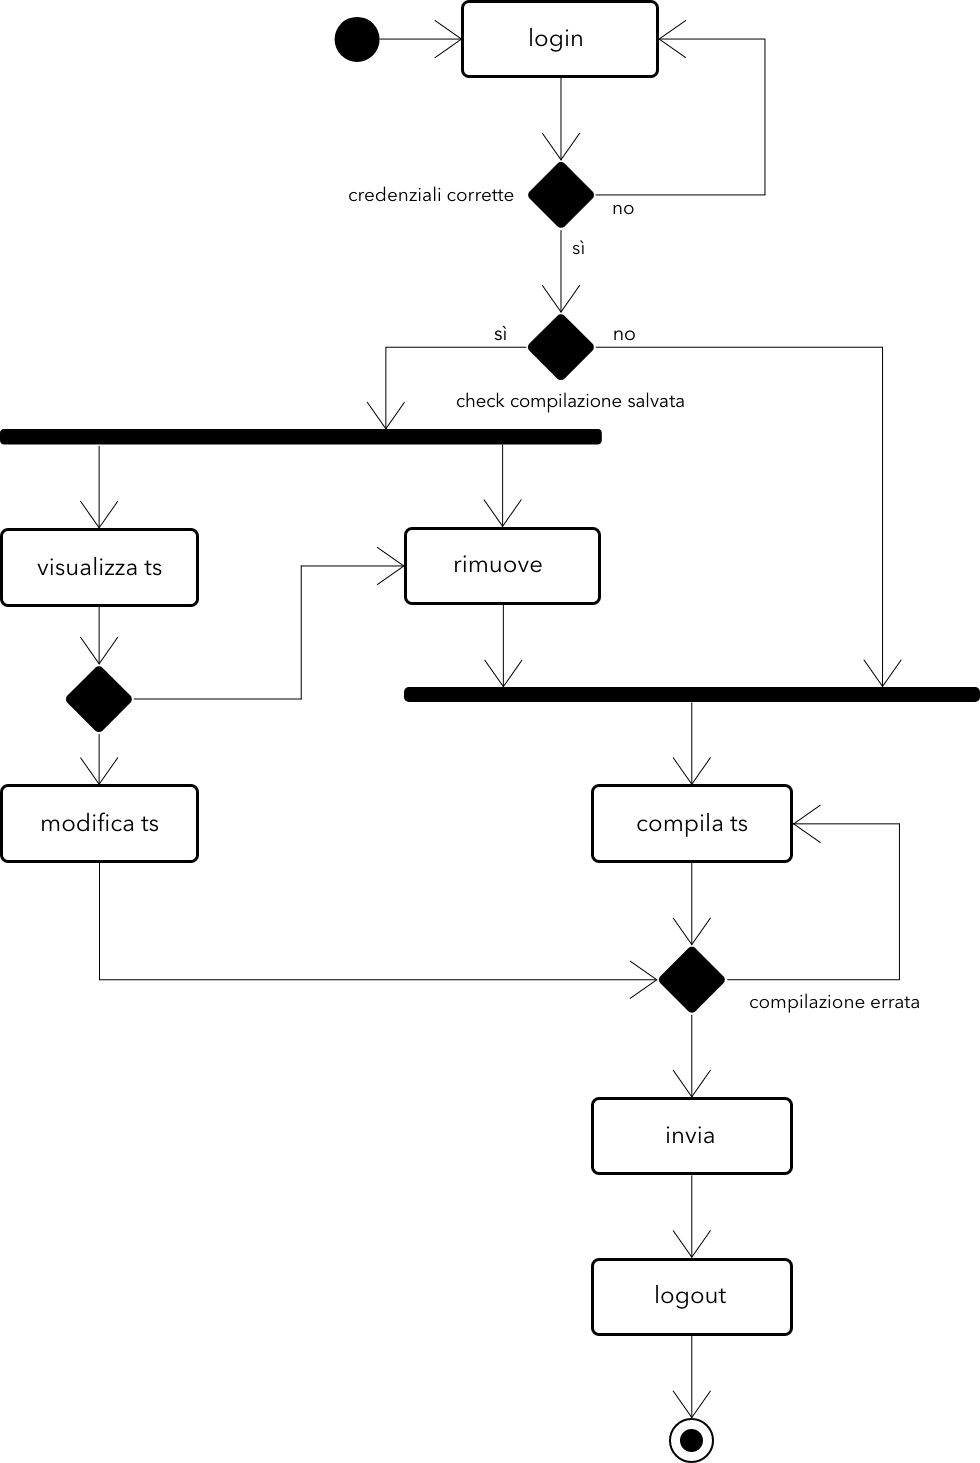
\includegraphics[width=.8\linewidth]{AD_Compila_ts.png}
	\caption{Diagramma di attività relativo alla compilazione del timesheet.}
	\label{fig:ad_compilats}
\end{figure}

\subsection{Verifica e approvazione del timesheet}
\textbf{Nome}: Controlla ts.\\
\textbf{Portata}: Tempo.\\
\textbf{Livello}: Obiettivo utente.\\
\textbf{Attore primario}: Manager.\\
\textbf{Parti interessate e interessi}: 
\begin{itemize}
    \item Manager, vuole approvare i timesheet inviati dai dipendenti, che siano conformi all'attività di lavoro svolta e compilati correttamente, al fine di completare le rendicontazione mensile.
    \item Impiegato, vuole la conferma sul timesheet al fine del calcolo del salario mensile.
\end{itemize}
\textbf{Pre-condizioni}: L'utente manager deve aver effettuato il login.\\
\textbf{Garanzia di successo}: Il manager segnala all'azienda di procedere con il calcolo del salario e delle imposte dovute. L’azienda emette il pagamento nei confronti del dipendente.\\
\textbf{Scenario principale di successo}
\begin{enumerate}
    \item Il manager entra nella sezione relativa ai timesheet inviati dai dipendenti.
    \item Il manager seleziona un timesheet e lo esamina.
    \item Il manager controlla che il codice commessa inserito sia corretto. 
    \item Il manager verifica che le ore giornaliere inserite siano coerenti con l'attività svolta dal dipendente.
    \item Il manager approva il timesheet.
    \item Il sistema registra i dati e mostra un messaggio di conferma.
    \item Il sistema rende disponibile il download del timesheet in formato Excel.
\end{enumerate}
\textbf{Estensioni}\\
5a. Il manager non approva il timesheet: 
\begin{enumerate}
    \item Il manager rigetta il timesheet del dipendente.
    \item Il sistema registra i dati e mostra un messaggio di conferma.
    \item Il sistema riabilita la modifica del timesheet nell'area personale del relativo dipendente.
\end{enumerate}

\begin{figure}[H]
    \vspace{2cm}
	\centering
	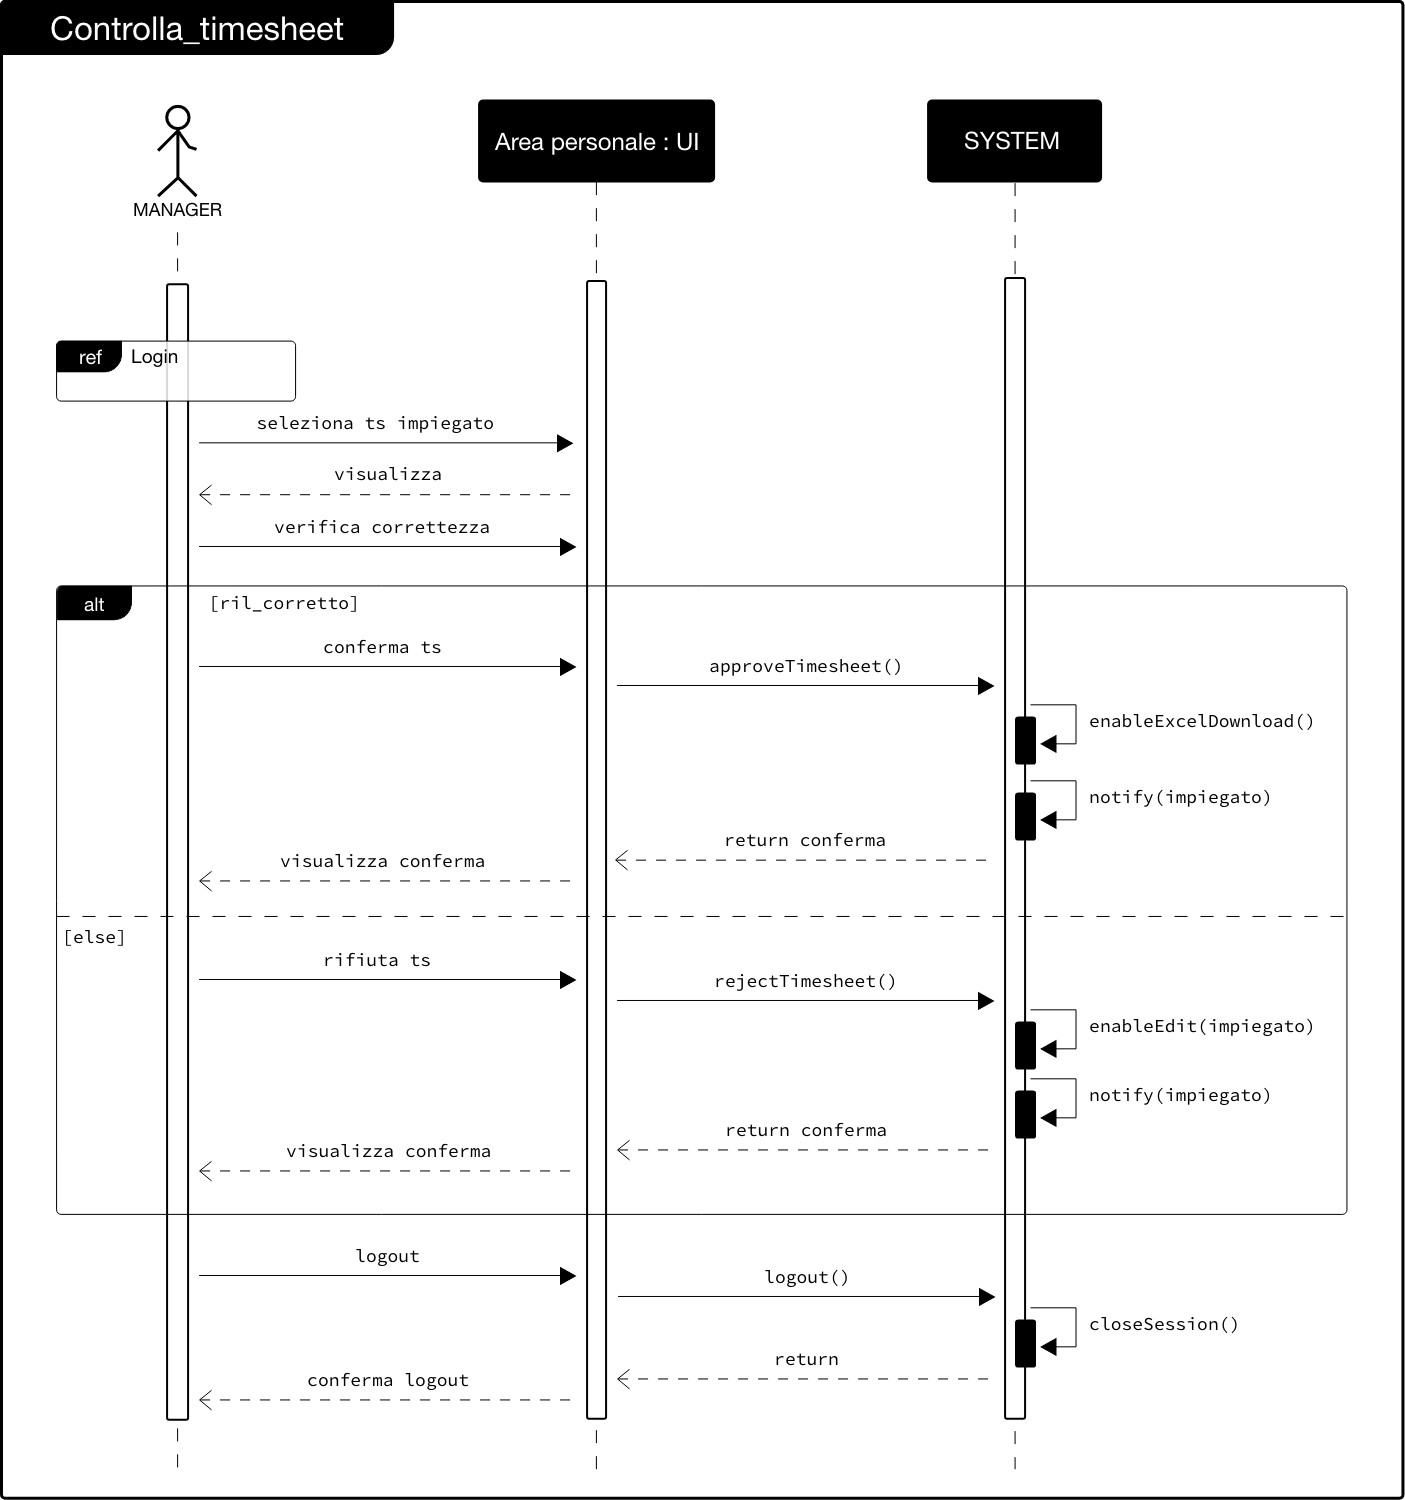
\includegraphics[width=1\linewidth]{SD_Controllo_ts.png}
	\caption{Diagramma di sequenza relativo al controllo del timesheet.}
	\label{fig:sd_controllots}
\end{figure}

\begin{figure}[H]
	\centering
	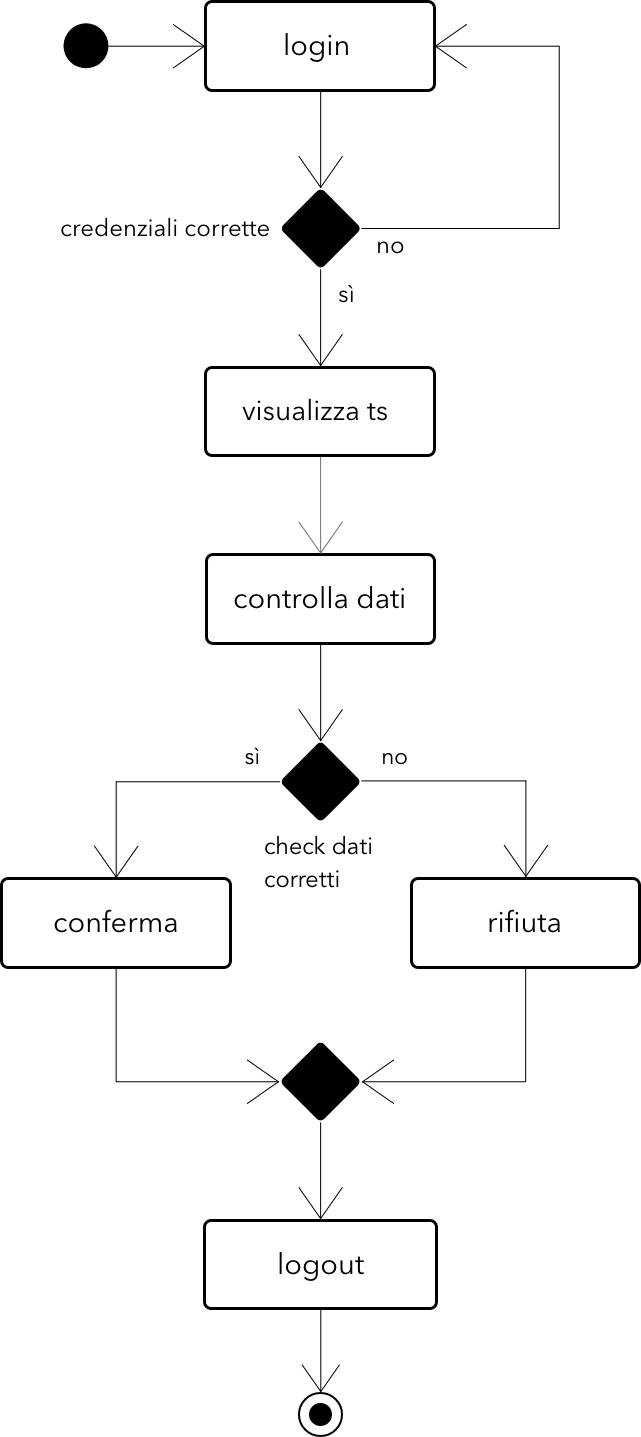
\includegraphics[width=.5\linewidth]{AD_Controllo_ts.png}
	\caption{Diagramma di attività relativo al controllo del timesheet.}
	\label{fig:ad_controllots}
\end{figure}

\subsection{Download del timesheet}
\textbf{Nome}: Scarica ts.\\
\textbf{Portata}: Tempo.\\
\textbf{Livello}: Obiettivo utente.\\
\textbf{Attore primario}: Impiegato, Manager, Azienda.\\
\textbf{Parti interessate e interessi}: Utente (Impiegato, Manager, Azienda), vuole scaricare localmente il timesheet.\\
\textbf{Pre-condizioni}: L’utente deve aver effettuato il login. Il timesheet deve esser stato approvato dal manager.\\
\textbf{Garanzia di successo}: L’utente possiede una copia in locale del timesheet.\\
\textbf{Scenario principale di successo}: 
\begin{enumerate}
    \item L’utente seleziona il mese di interesse.
    \item L'utente verifica lo stato del timesheet.
    \item L'utente effettua il download del timesheet in formato Excel.
\end{enumerate}

\section{Requisiti non funzionali}
L'accesso all'area personale viene eseguito attraverso una pagina di login apposita. \\
Per quanto riguarda i ruoli, il sistema deve prevedere tre livelli di accesso differenti: 
\begin{itemize}
    \item \textit{master}, pensato come utenza aziendale globale, a cui è consentito effettuare qualsiasi tipo di operazione messa a disposizione dall'applicazione e che ha visibilità totale dei dati;
    \item \textit{manager}, pensato per il responsabile di sede e attraverso cui si ha visibilità sulla rendicontazione dei singoli dipendenti, relativi a quella specifica sede. Tale utenza viene creata dall'utente master;
    \item \textit{employee}, utenza di base pensata per il dipendente e la quale dà accesso alle sole informazioni personali. Questo tipo di utenza deve essere creata dall'utente master oppure dal manager di sede relativo.
\end{itemize}
Una volta effettuata l'autenticazione il sistema visualizza la pagina principale, contente il timesheet di lavoro del mese corrente, un calendario e una sezione dedicata alle notifiche. La rappresentazione del timesheet viene effettuata tramite una tabella, la quale comprende le seguenti colonne: codice commessa, data, numero di ore lavorate, numero di ore di permesso/ferie e infine un campo per indicare l'assenza per malattia. \\
Al momento del salvataggio dei dati inseriti o dell'invio del timesheet, il sistema deve mostrare una conferma di avvenuta operazione oppure un errore se non è stato possibile eseguire l'azione richiesta.